\documentclass[a4paper,ngerman,12pt]{scrartcl}

\usepackage[utf8]{inputenc}
%\usepackage[ansinew]{inputenc}

\usepackage[ngerman]{babel}

\usepackage{amsmath,amsthm,amssymb,stmaryrd,color,graphicx}
\usepackage{setspace}
\usepackage{bussproofs}
\usepackage{array}
\usepackage{comment}
\usepackage{wrapfig}

\usepackage{enumitem}

\usepackage{units}

\usepackage[protrusion=true,expansion=true]{microtype}

\usepackage{lmodern}

\usepackage{hyperref}
\usepackage{cleveref}

\newcommand{\RR}{\mathbb{R}}
\newcommand{\CC}{\mathbb{C}}
\newcommand{\ZZ}{\mathbb{Z}}
\newcommand{\NN}{\mathbb{N}}
\newcommand{\QQ}{\mathbb{Q}}

\newcommand{\red}[1]{{\color{red}#1}}

\setlength\parskip{\medskipamount}
\setlength\parindent{0pt}

\theoremstyle{definition}
\newtheorem{defn}{Definition}[]
\newtheorem{axiom}[defn]{Axiom}
\newtheorem{bsp}[defn]{Beispiel}

\theoremstyle{plain}
\newtheorem{prop}[defn]{Proposition}
\newtheorem{motto}[defn]{Motto}
\newtheorem{wunder}[defn]{Wunder}
\newtheorem{ueberlegung}[defn]{Überlegung}
\newtheorem{lemma}[defn]{Lemma}
\newtheorem{kor}[defn]{Korollar}
\newtheorem{hilfsaussage}[defn]{Hilfsaussage}
\newtheorem{satz}[defn]{Satz}
\newtheorem{frage}[defn]{Frage}

\theoremstyle{remark}
\newtheorem{bem}[defn]{Bemerkung}
\newtheorem{aufg}[defn]{Aufgabe}

\newtheorem*{antwort}{Antwort}

\newlength{\aufgabenskip}
\setlength{\aufgabenskip}{1.4em}
\newcounter{aufgabennummer}
\newenvironment{aufgabe}[1]{
	\addtocounter{aufgabennummer}{1}
	\textbf{Aufgabe \theaufgabennummer.} \emph{#1} \par
}{\vspace{\aufgabenskip}}

\clubpenalty=10000
\widowpenalty=10000
\displaywidowpenalty=10000

\setlength\unitlength{1cm}

\usepackage{tikz}

\RequirePackage{geometry}
\geometry{textwidth=16.0cm,textheight=24.5cm,footskip=1.5cm}

\begin{document}
	
\begin{picture}(0,0)
\put(0,-0.5){%
	
\includegraphics[scale=0.1]{logo-ifm}
}
\put(14.0,-3.5){%
	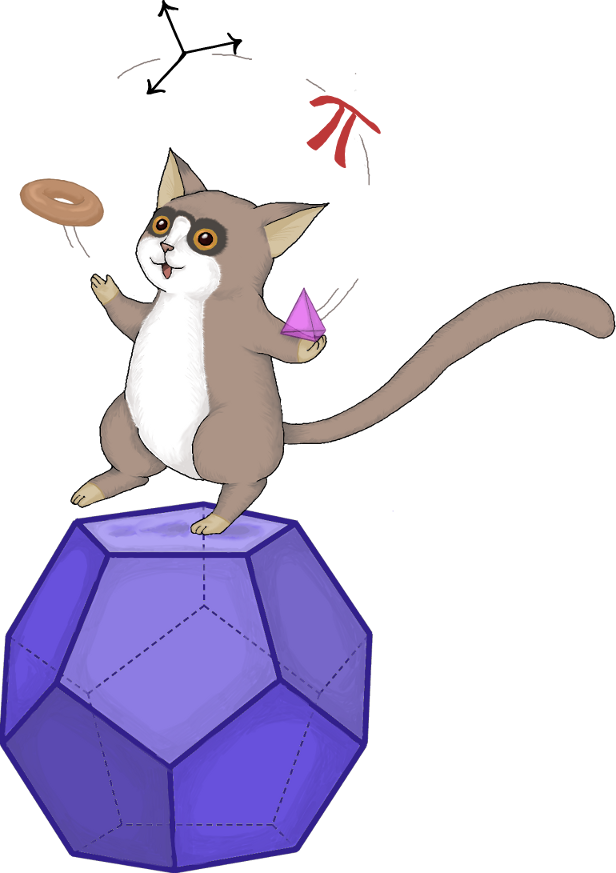
\includegraphics[scale=0.17]{cover}
}
\end{picture} 
	
\vspace{6em}

\begin{center}\Large{Siebter Korrespondenzbrief}\end{center}

\section*{Codierungstheorie}

Erinnerst du dich noch an den Korrespondenzbrief zum Thema \glqq Kryptographie\grqq{} (Brief~4)? In dem ging es darum eine Nachricht so zwischen zwei Personen auszutauschen, dass niemand anders diese Nachricht verstehen kann.

In aktuellen Brief geht es nun ebenfalls darum, dass zwei Personen eine Nachricht austauschen wollen. Diesmal ist deren Sorge aber nicht, dass jemand anders die Nachricht lesen könnte, sondern dass die Nachricht beim Übertragen verfälscht wird. Das kann zum Beispiel passieren, wenn die Leitung, über die die Nachricht übertragen wird, kleinere Defekte aufweist. Oder wenn die Nachricht über eine weite Strecke übertragen werden muss.

Der Sender der Nachricht möchte daher seine Nachricht auf eine solche Weise \emph{codieren}, dass der Empfänger es erkennen kann, wenn die Nachricht beim Übertragen verfälscht wurde. Dieses Ziel auf eine möglichst effiziente Weise zu erreichen ist das Thema der \glqq Codierungstheorie\grqq.


\section{Einführung}

Eine besonders einfache Methode Fehler bei der Übertragung zu erkennen, ist die Folgende: Man sendet die zu übertragende Nachricht einfach zweimal hintereinander. Passiert beim Übertragen der Nachricht ein Fehler, so erkennt der Empfänger das daran, dass die beiden Hälften der Nachricht nicht mehr gleich sind.

\begin{bsp}	
	Wollen wir bspw. das Wort \texttt{JUNI} übertragen, so senden wir stattdessen das Codewort \texttt{JUNIJUNI}. Passiert beim Übertragen ein einzelner Fehler (ein Buchstabe wird verfälscht), so erhält der Empfänger bspw. das Wort \texttt{JU\red{L}IJUNI} und kann direkt sehen, dass ein Fehler passiert sein muss.
\end{bsp}

Wir können es also erkennen, wenn bei der Übertragung ein Fehler passiert - wir können diesen Fehler aber nicht korrigieren (denn wir wissen ja nicht welche der beiden Hälften des Codewortes die korrekte ist). Außerdem können wir nur dann sicher sein, Fehler zu erkennen, wenn höchstens ein Fehler passiert. Treten bei der Übertragung zwei oder mehr Fehler auf, so kann es passieren, dass der Empfänger das nicht mehr erkennen kann:
	\begin{center}
		\texttt{JUNIJUNI} $\xrightarrow{\hspace*{2cm}}$ \texttt{JU\red{L}IJU\red{L}I}
	\end{center}

\begin{aufgabe}{}\label{aufgabe:verdreifachungsCodierung}
	Kannst du das Verfahren so anpassen, dass er auch zwei Fehler noch in jedem Fall erkennen kann?
	
	Kannst du das oben beschriebene Verfahren so anpassen, dass ein einzelner Fehler vom Empfänger nicht nur erkannt, sondern auch korrigiert werden kann?
\end{aufgabe}

Diese einfachen Codierungsverfahren funktionieren zwar grundsätzlich, haben aber einen großen Nachteil. Die zu übertragenden Codes werden erheblich größer als die eigentliche Nachricht. Ein zentrales Ziel der Codierungstheorie ist es daher möglichst \emph{effiziente} Codierungsverfahren zu finden, die die Nachrichten nur ein wenig größer machen, aber es trotzdem erlauben Fehler zu erkennen (und evtl. sogar zu korrigieren).

Bevor wir uns auf die Suche nach solchen Verfahren machen können, müssen wir erst noch genauer festlegen, wie wir die Effizienz eines Codierungsverfahrens bestimmen wollen. Dazu werden wir ab sofort nur noch Verfahren der folgenden Form betrachten: 
\begin{enumerate}
	\item Teile die zu übertragende Nachricht in Stücke gleicher Länge ein. Diese Stücke nennen wir \emph{Wörter}. 
	\item Ersetze jedes der Wörter durch ein ihm zugeordnetes \emph{Codewort} - diese Codewörter müssen dabei ebenfalls alle eine einheitliche Länge haben.
	\item Schreibe die Codewörter wieder hintereinander und erhalte so die zu übertragende Nachricht.
\end{enumerate}

\begin{bsp}\label{bsp:Verdopplungscodierung}
	Wollen wir zum Beispiel die Verdopplungscodierung von oben mit einer Wortlänge von $4$ anwenden, um die Nachricht \texttt{DIESISTEINETESTNACHRICHT} zu übertragen, so funktionieren die Schritte wie folgt:
	\begin{enumerate}
		\item Teile die Nachricht in Wörter der Länge $4$: \texttt{DIES ISTE INET ESTN ACHR ICHT}
		\item Ersetze die Wörter durch ihre Codewörter: \texttt{DIES} $\rightarrow$ \texttt{DIESDIES}, \texttt{ISTE} $\rightarrow$ \texttt{ISTEISTE}
		\item Erhalte die codierte Nachricht:	
		 \begin{center}
		 	\texttt{DIESDIESISTEISTEINETINETESTNESTNACHRNACHRICHTICHT}
		 \end{center}
	\end{enumerate}
\end{bsp}

\begin{bem}
	Tatsächlich werden wir uns für den Rest dieses Briefes nun nur noch damit beschäftigen, wie man ein einzelnes Nachrichtenwort codiert (und wieder decodiert). Möchte man längere Nachrichten übertragen, kann man die Nachricht dann schließlich immer wie oben beschrieben in kürzerer Wörter zerlegen und einzeln codieren.
\end{bem}

Für Verfahren der oben beschriebenen Form, können wir nun ganz einfach bestimmen, wie effizient sie sind:

\begin{defn}
	Als \emph{Informationsrate} eines bestimmten Codierungsverfahrens bezeichnet man das Verhältnis aus der Länge der Codewörter zur Länge der Nachrichtenwörter, also die Zahl
		\[\frac{\text{Länge eines Codewortes}}{\text{Länge eines Nachrichtenwortes}}\]
	Je kleiner diese Zahl ist, desto effizienter ist das Verfahren.
\end{defn}

\begin{bsp}
	Für das Verdopplungscodierungsverfahren aus \Cref*{bsp:Verdopplungscodierung} ist die Informationsrate also:
		\[\frac{\text{Länge eines Codewortes}}{\text{Länge eines Nachrichtenwortes}} = \frac{8}{4} = 2\]
	Eine mit diesem Verfahren codierte Nachricht benötigt also doppelt so viel Platz wie die ursprüngliche Nachricht.
\end{bsp}

\begin{aufgabe}{}\label{aufgabe:verdreifachungsCodierungIR}
	Bestimme die Informationsrate für deine in Aufgabe 1 gefundenen Verfahren.
\end{aufgabe}

Als weitere Vereinfachung werden wir im restlichen Brief nur noch Nachrichten (und Codierungen) betrachten, die ausschließlich aus Zahlen bestehen. Das ist aber keine wirkliche Einschränkung, denn wie du schon im Kryptographie-Brief gesehen hast, lassen sich Buchstaben auch leicht durch Zahlen darstellen.


\section{Fehlererkennung}

Als erstes wollen wir uns nun mit Verfahren beschäftigen, die es uns erlauben einzelne Fehler zu erkennen. Das Verfahren soll dabei die folgende Form haben: Wir nehmen das Wort aus der Nachricht und codieren es, indem wir noch \glqq irgendetwas\grqq{} daran anhängen. Dieses \glqq irgendetwas\grqq{} soll es dem Empfänger dann erlauben einen möglicherweise aufgetretenen Fehler zu erkennen.
	\begin{center}
		\texttt{1847} $\xrightarrow{\text{Codierung}}$ \texttt{1847\_\_\_}
	\end{center}

Im ersten Kapitel war dieses \glqq irgendetwas\grqq{} zum Beispiel einfach wieder das Wort selbst. Das ist aber ziemlich ineffizient, da das Wort dadurch gleich doppelt so lang wird. Besser wäre es da beispielsweise nur die Quersumme des Wortes (das ist die Summe der einzelnen Ziffern) anzuhängen. Sind die Wörter vier Ziffern lang, so kann die Quersumme höchstens $9+9+9+9=36$ sein - uns genügt also ein zweistelliges Anhängsel.

\begin{bsp}
	Wollen wir die Nachricht $1701$ übertragen, so bilden wir die Quersumme $1+7+0+1=9$ und erhalten damit das Codewort $1701\textbf{09}$. Passiert beim Übertragen nun ein Fehler, so erhält der Empfänger beispielsweise die Nachricht $\red{8}70109$. Dieser kann nun leicht erkennen, ob ein Fehler aufgetreten ist, indem er einfach wieder die Quersumme der ersten vier Ziffern bildet ($8+7+0+1=16$) und mit den letzten beiden Ziffern vergleicht. Stimmen diese beiden Zahlen nicht überein, so weiß der Empfänger, dass beim Übertragen ein Fehler passiert sein muss.
\end{bsp}

\begin{aufgabe}{}
	Du bist der Empfänger und erhältst die folgenden Codewörter (die ursprünglichen Wörter hatten die Länge $4$):
		\[172919 \quad-\quad 422416 \quad-\quad 939124  \quad-\quad 314109\]
	Prüfe für jedes der Wörter, ob beim Übertragen ein Fehler aufgetreten ist. Falls nein, gib das ursprüngliche (uncodierte) Wort an. Falls ja, gib zwei Möglichkeiten an, wie das ursprüngliche Wort gelautet haben könnte (unter der Annahme, dass bei der Übertragung höchstens eine Ziffer verändert wurde). 
	
	Bei folgendem Codewort, ist bei der Übertragung etwas spezielles passiert - kannst du erklären was?
		\[739150\]
\end{aufgabe}

Funktioniert dieses Verfahren auch? D.h. können wir damit wirklich jeden einzeln auftretenden Fehler erkennen? Ja, das können wir - denn wann immer eine einzelne Ziffer verändert wird, so ändert sich auch die Quersumme der ganzen Zahl. 

Ist das Verfahren effizient? Nun, die Informationsrate ist $\frac{\text{Länge eines Codewortes}}{\text{Länge eines Nachrichtenwortes}} = \frac{6}{4} = 1,5$ - also auf jeden Fall schonmal besser als bei dem bisherigen Verfahren.

Tatsächlich geht es aber sogar noch besser: Denn wenn nur eine einzelne Ziffer in der Nachricht verfälscht wird, dann kann sich die Quersumme doch höchstens um $9$ verändern. Es genügt also völlig, wenn wir uns nur die Einerstelle der Quersumme merken (oder anders ausgedrückt: Den Rest der Quersumme bei Division durch $10$). Diese Ziffer am Ende der eigentlichen Nachricht wird oft als \emph{Prüfziffer} bezeichnet (da man mit ihr prüfen kann, ob die Nachricht korrekt übertragen wurde).

\begin{bsp}
	Um mit diesem Verfahren die Nachricht $8245$ zu übertragen, bilden wir also erneut die Quersumme $8+2+4+5=19$ und nehmen deren Einerstelle $9$. So erhalten wir das Codewort $8245\textbf{9}$.
\end{bsp}

\begin{aufgabe}{}
	Du empfängst die folgenden Codewörter - bei welchen von ihnen muss ein Fehler bei der Übertragung passiert sein?
		\[23836 \quad-\quad 99999 \quad-\quad 47629 \quad-\quad 38425\]
\end{aufgabe}

\begin{aufgabe}{}
	Bestimme die Informationsrate dieses Codierungsverfahrens.

	\emph{Zusatzaufgabe:} Kannst du das Verfahren irgendwie so verändern, dass die Informationsrate noch niedriger wird?
\end{aufgabe}


Ein mit diesem System sehr eng verwandtes Verfahren wird für die ISBN (\emph{Internationale Standardbuchnummer}) verwendet - einer $13$-stelligen Nummer\footnote{Bis 2007 gab es eine andere, $10$-stellige Variante der ISBN - sie funktioniert im Wesentlichen genauso wie die neue ISBN, hat aber ein leicht anderes Verfahren zur Berechnung der Prüfziffer.}, mit deren Hilfe Bücher eindeutig identifiziert werden können (z.B. wenn man sie in einem Buchladen bestellen will). Die ISBN findest du oft auf einer der ersten Buchseiten oder auf der Rückseite zusammen mit dem Barcode.

Die Nummer selbst besteht dabei aus den ersten $12$ Ziffern, die letzte Ziffer ist wieder eine Prüfziffer. Um diese Prüfziffer zu bilden, berechnen wir eine Art Quersumme - multiplizieren dabei aber zuvor noch jede zweite Ziffer mit $3$. Dies sieht dann zum Beispiel so aus:

\begin{center}
	\begin{tabular}{ccccccccccccccccc}
		1 & 2 & 3 & - & 4 & - & 5 & 6 & - & 7 & 8 & 9 & 0 & 1 & 2 & & \\
		$\downarrow$ & $\downarrow$ & $\downarrow$ & & $\downarrow$ & & $\downarrow$ & $\downarrow$ & & $\downarrow$ & $\downarrow$ & $\downarrow$ & $\downarrow$ & $\downarrow$ & $\downarrow$ & & \\
		1 & 6 & 3 & & 12 & & 5 & 18 & & 7 & 24 & 9 & 0 & 1 & 6 & $\Rightarrow$ & \textbf{192}
	\end{tabular}
\end{center}

Die eigentliche Prüfziffer erhalten wir dann, indem wir schauen wie viel von der berechneten Zahl noch bis zur nächsten vollen Zehnerzahl fehlt (im obigen Beispiel also $8$). Anders gesagt: Wir wählen die Prüfziffer gerade so, dass die abgewandelte Quersumme der vollständigen $13$-stelligen ISBN eine Zehnerzahl ist. 

Wenn man eine angebliche ISBN genannt bekommt, muss man also nur prüfen, ob die abgewandelte Quersumme einer Zehnerzahl ist - wenn das nicht der Fall ist, muss die Nummer fehlerhaft sein.

\begin{aufgabe}{}
	Ich habe von drei Büchern in meinem Zimmer die ISBN abgetippt - bei welchen der Nummern ist mir dabei ein Fehler unterlaufen?
	\begin{center}
		978-349805241-6 \quad-\quad 978-357003412-9 \quad-\quad 978-184854956-2
	\end{center}
\end{aufgabe}

\begin{aufgabe}{}
	Bestimme die Informationsrate von ISBN.
\end{aufgabe}

Nun wissen wir also wie das Codierungsverfahren der ISBN funktioniert. Aber welche Fehler kann man damit erkennen? 

Zunächst einmal kann man hier wieder alle Einzelfehler erkennen, d.h. wenn eine einzelne Ziffer der ganzen Zahl verfälscht wurde. Bei den Stellen, die unverändert in die Quersumme aufgenommen werden, ist das recht klar - denn hier gilt einfach das gleiche wie bei dem Verfahren vom Beginn dieses Kapitels. Was aber ist mit den Stellen, an denen die Ziffer zunächst mit $3$ multipliziert wird?

\begin{center}
	\begin{tabular}{cccccccccc}
		0 & 1 & 2 & 3 & 4 & 5 & 6 & 7 & 8 & 9 \\
		$\downarrow$ & $\downarrow$ & $\downarrow$ & $\downarrow$ & $\downarrow$ & $\downarrow$ & $\downarrow$ & $\downarrow$ & $\downarrow$ & $\downarrow$ \\
		0 & 3 & 6 & 9 & 12 & 15 & 18 & 21 & 24 & 27
	\end{tabular}
\end{center}

Nun, wie du an obiger Tabelle sehen kannst, führt das Multiplizieren mit $3$ dazu, dass zwei verschiedene Ziffern zu zwei Zahlen werden, die immer noch zwei verschiedene Einerstellen haben. Und für die Prüfziffer sind am Ende nur die Einerstellen wichtig. Also können wir auch hier jede Veränderung einer einzelnen Ziffer anhand der Prüfziffer feststellen.

\begin{aufgabe}{Warum ausgerechnet 3?}
	Statt jede zweite Ziffer mit $3$ zu multiplizieren, könnte man ja beispielsweise auch jede zweite Ziffer mit $2$ multiplizieren. Kannst du dir vorstellen, warum tatsächlich aber die $3$ statt der $2$ gewählt wurde? 
	
	\emph{Tipp:} Schreibe dir dazu eine Tabelle für Multiplikation mit $2$ wie die oben für Multiplikation mit $3$ auf. Überlege dir dann, ob das obige Argument für die Korrektheit des Verfahren immer noch richtig ist.
	
	Kannst du eine andere Zahl finden, die man statt der $3$ verwenden könnte (und die eine genauso gute Fehlererkennung ermöglichen würde)?
\end{aufgabe}

Das Codierungsverfahren der ISBN ist also zumindest schon mal so gut wie das vom Anfang dieses Kapitels. Tatsächlich ist es aber sogar noch ein wenig besser! Es kann nämlich noch eine weitere Fehlerart erkennen, die gerade beim Eintippen von Zahlen oft passiert: Das Vertauschen zweier benachbarten Ziffern. Wenn man also zum Beispiel statt $12345$ die Zahl $1\red{32}45$ eingibt.

\begin{bsp}
	Wir betrachten als Beispiel die folgende $12$-stellige Nummer (noch ohne Prüfziffer): $140011000000$
	
	Dann erhalten wir als abgewandelte Quersumme $1+3\cdot 4+0+3\cdot 0+1+3\cdot 1+ 0+\dots +0=17$ und folglich als Prüfziffer die $3$.
	
	Vertauschen wir aber die ersten beiden Ziffern, so erhalten wir die Nummer $\red{41}0011000000$ mit abgewandelter Quersumme $4+3\cdot 1 + \dots = 11$ und damit der Prüfziffer $9$.
	
	Das Vertauschen zweier benachbarter Ziffern führt also tatsächlich zu unterschiedlichen Prüfziffern.
\end{bsp}

Dieses Erkennen von Ziffernvertauschungen ist also der Grund, warum für die ISBN die abgewandelte Quersumme zur Berechnung der Prüfziffer verwendet wird. Leider ist dieses Verfahren aber nicht ganz perfekt. Es gibt nämlich einige wenige Paare von Ziffern, bei denen sich die Quersumme nicht ändert, wenn man diese beiden Ziffern vertauscht. 

Ein Beispiel für ein solches Ziffernpaar sind $1$ und $6$. Beginnt eine ISBN mit der Folge $16$, so trägt dies $1+3\cdot 6=19$  zur abgewandelten Quersumme bei. Vertauscht man die beiden Ziffern, erhält man den Anfang $61$, welcher $6+3\cdot 1=9$ zur abgewandelten Quersumme beiträgt. Diese beiden Zahlen sind zwar nicht gleich, sie haben aber die gleiche Einerstelle und führen daher zur gleichen Prüfziffer. Also können wir es nicht erkennen, wenn wir beim Abtippen einer ISBN die zwei benachbarten Ziffern $1$ und $6$ vertauschen.

\begin{aufgabe}{Andere Problempaare}
	Kannst du noch weitere Ziffernpaar finden, deren Vertauschung wir ebenfalls nicht erkennen können?
	
	\emph{Zusatzaufgabe:} Kannst du \emph{alle} solchen Paare finden und begründen, warum dies auch wirklich alle sind?
\end{aufgabe}


%\begin{aufgabe}{Geldscheine}
%	Prüfziffer auf Euroscheinen...
%\end{aufgabe}

\newpage
\section{Fehlerkorrektur}

Zum Schluss wollen wir nun noch ein Codierungsverfahren kennen lernen, bei dem der Empfänger einen einzelnen Fehler nicht nur erkennen, sondern ihn sogar wieder verbessern kann. Um das zu erreichen müssen wir also sicherstellen, dass der Empfänger nicht nur herausfinden kann, \emph{dass} beim Übertragen ein Fehler passiert ist, sondern auch noch \emph{an welcher Stelle} der Nachricht der Fehler passiert ist.

Dazu benötigen wir nun mehr als nur eine einzelne Prüfziffer! Das Verfahren, das wir betrachten wollen, verwendet dazu gleich vier Prüfziffern für ein Nachrichtenwort, das selbst aus vier Ziffern besteht. Konkret funktioniert die Codierung dann wie folgt:

\begin{enumerate}
	\item Nimm das Nachrichtenwort und schreibe es in ein Quadrat:
		\[7185 \xrightarrow{\hspace{2em}} \begin{array}{cc}7 & 1 \\8 & 5\end{array}\]
	\item Berechne für jede Zeile und jede Spalte eine eigene Prüfsumme (normale Quersumme, dann Rest bei Division durch $10$) und schreibe diese rechts neben die jeweilige Zeile bzw. unter die entsprechende Zeile:
		\[\begin{array}{cc}7 & 1 \\8 & 5\end{array} \xrightarrow{\text{Berechnen der Prüfziffern}} \begin{array}{ccc}7 & 1 & 8\\8 & 5 & 3 \\ 5 & 6 &\end{array}\]
	\item Passiert nun beim Übertragen ein Fehler, so werden dadurch gleich zwei Prüfsummen falsch (eine für die entsprechende Spalte und eine für die entsprechende Zeile). Dadurch kann der Empfänger erschließen, an welcher Stelle der Fehler passiert sein muss und kann diese Stelle so verbessern, dass die Prüfsummen wieder korrekt sind:
		\[\begin{array}{ccc}7 & 1 & 8\\8 & 5 & 3 \\ 5 & 6 &\end{array} \xrightarrow{\text{Übertragung (Fehler bei 8)}} \begin{array}{ccc}7 & 1 & 8\\5 & 5 & {\color{red}3} \\ {\color{red}5} & 6 &\end{array}\]
\end{enumerate}

\begin{aufgabe}{}
	Du erhältst folgende Nachrichten. Prüfe bei welcher davon ein Fehler passiert sein muss und korrigiere diesen:
		\[\begin{array}{ccc}3 & 5 & 8\\1 & 2 & 6 \\ 4 & 0 &\end{array} \quad-\quad \begin{array}{ccc}9 & 9 & 8\\6 & 1 & 3 \\ 5 & 6 &\end{array} \quad-\quad \begin{array}{ccc}4 & 3 & 7\\3 & 8 & 1 \\ 7 & 1 &\end{array}\]
\end{aufgabe}

\begin{aufgabe}{}
	Bestimme die Informationsrate dieses Codierungsverfahrens.
	
	Beschreibe ein ganz ähnliches Codierungsverfahren für Nachrichtenworte der Länge $9$. Was ist hierbei die Informationsrate?
\end{aufgabe}

\begin{aufgabe}{}
	Genau genommen habe ich bei der Beschreibung des Codierungsverfahrens oben ein wenig geschummelt: Bei der Fehlererkennung habe ich nämlich so getan als könnten Fehler nur im ursprünglichen Nachrichtenwort auftreten. Tatsächlich kann aber natürlich genauso gut eine der Prüfziffern beim Übertragen verfälscht werden. 
	
	Kann der Empfänger auch solch einen Fehler erkennen und beheben (also einen Fehler, bei dem also eine einzelne Prüfsumme verfälscht wurde, der Rest der Nachricht aber korrekt geblieben ist)? Und wenn ja, wie?
\end{aufgabe}

\end{document}